\chapter{Lyrics Retrieval and Alignment} \label{chap:retrieval_alignment}

Lyrics retrieval and alignment are related tasks: The retrieval task can be interpreted as an alignment of all possible lyrics sequences to the query audio, and a subsequent selection of the best-matching result. This is done in all described algorithms.\\
As a starting point, a traditional HMM-based algorithm for Forced Alignment was tested. Building on top of the posteriorgrams extracted with the new acoustic models as described in chapter \ref{chap:phonerec}, a new algorithm using Dynamic Time Warping (DTW) was developed and evaluated for both alignment and retrieval. Next, another processing step for explicitly extracting phonemes from the posteriorgrams was included; the resulting method was also tested for both alignment and retrieval. All three mentioned algorithms were entered into the 2017 \textit{MIREX} challenge for lyrics-to-audio alignment, in which the algorithms were tested on Hansen's dataset, both in the singing-only and polyphonic conditions (\textit{ACAP} and \textit{ACAP\_Poly}, see sections \ref{subsec:data_hansen} and \ref{subsec:data_hansen_polyphonic}), and on Mauch's alignment data set (\textit{Mauch}, see section \ref{subsec:data_mauch_alignment}). The results can be viewed on \url{http://www.music-ir.org/mirex/wiki/2017:Automatic_Lyrics-to-Audio_Alignment_Results} (last checked: ???).\\
Finally, a practical application for lyrics alignment is presented: Automatic expletive detection in rap songs.


\section{HMM-based lyrics-to-audio alignment}\label{sec:ret_hmm}
For this algorithm, monophone Hidden Markov Models were trained on the \textit{TIMIT} speech data using the HTK framework \cite{htk}. Then, Viterbi alignment was run to align the phonemes to the singing audio. These are the same models used to align lyrics to the \textit{DAMP} audio data to generate the training data set described in section \ref{sec:phonerec_acap}. The results in the \textit{MIREX} challenge are shown in figure \ref{fig:results_align_hmm}.
%TODO erkl�ren
\begin{figure}
 \begin{center}
                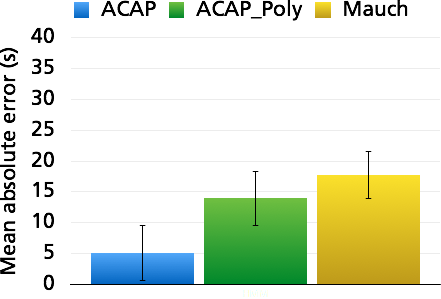
\includegraphics[width=0.8\textwidth]{images/res_align_hmm.png}
               \caption{\textit{MIREX} results on all three data sets using the HMM-based approach.}
                \label{fig:results_align_hmm}
                 \end{center}
 \end{figure}


\section{Posteriorgram-based retrieval and alignment}\label{sec:ret_post}

\begin{figure}
 \begin{center}
                \includegraphics[width=0.8\textwidth]{images/retrieval_dtw_process.png}
                \caption{Overview of the DTW-based lyrics alignment and retrieval method.}
                \label{fig:retrieval_dtw_process}
                 \end{center}
 \end{figure}

A new approach is based on the posteriorgrams generated with the DNN acoustic models described in section \ref{sec:phonerec_acap}; an overview is illustrated in figure \ref{fig:retrieval_dtw_process}. In order to align lyrics to these posteriorgrams, binary templates are generated from the text lyrics on the phoneme scale. These can be seen as oracle posteriorgrams, but do not include any timing information.\\
Between this template and the query posteriogram, a similarity matrix is calculated using the cosine distance. On the resulting matrix, Dynamic Time Warping (DTW) is then performed using the implementation from \cite{ellis_dtw} to obtain the alignment. An example is shown in figure \ref{fig:retrieval_dtw}.\\
Two optimizations were made to the algorithm. The first one was a sub-sampling of the phoneme posteriorgrams by the factor 10 (specifically, the mean for 10 consecutive frames was calculated). This increased the speed of the DTW for the individual comparisons and also produced better results. Longer windows were also tested, but this had a negative impact on the result.\\
Secondly, squaring the posteriorgrams before the similarity calculation produced slightly better results. This makes the posteriorgrams more similar to the binary lyrics templates used for comparison. Binarizing them was also tested, but this emphasized phoneme recognition errors too much.\\

In the retrieval case, the binary templates are generated for all possible lyrics in the database, and the DTW calculation is performed for each of them with the query posteriorgram. The DTW cost is used as the measure to obtain the best-matching lyrics. Since the phoneme durations in the actual recording and the lyrics templates have different lengths, the length of the warping path should not be a detrimental factor in cost calculation. 
Therefore, the accumulative cost of the best path is divided by the path length and then retained as a score for each possible lyrics document. In the end, the lyrics document with the lowest cost is chosen as a match (or, in some experiments, the N documents with the lowest costs).\\
As an additional experiment, both the textual lyrics corpus and the sung inputs were split into smaller segments roughly corresponding to one line in the lyrics each (around 12,000 lines). The retrieval process was then repeated for these inputs. This allowed an evaluation as to how well lyrics could be retrieved from just one single sung line of the song. (Sub-sequence DTW could also be used for this task instead of splitting both corpora.)\\


\begin{figure}
	\centering
	\begin{subfigure}[t]{0.3\textwidth}
		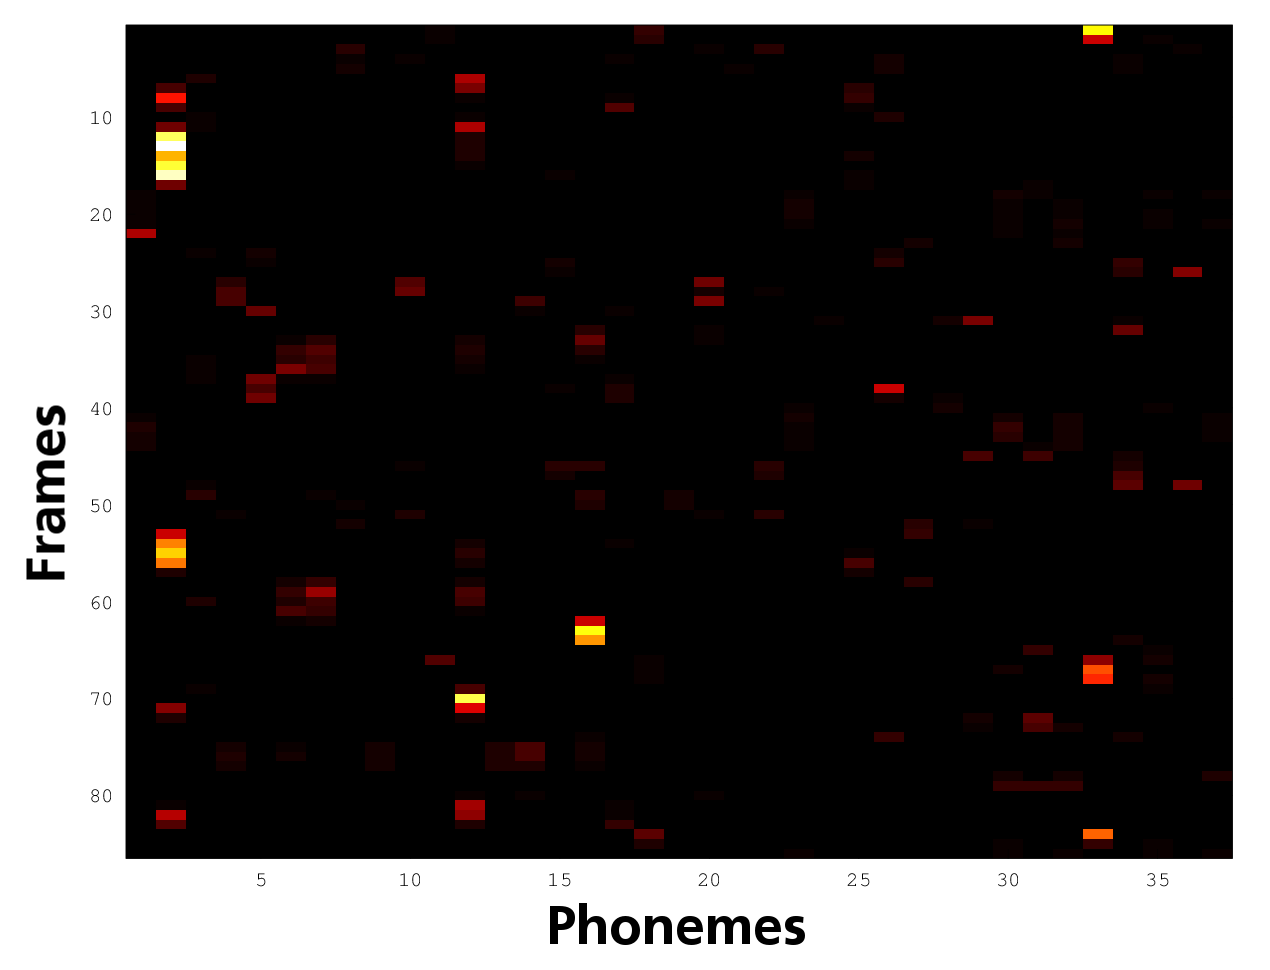
\includegraphics[width=\textwidth]{images/retrieval_posts.png}
		\caption{Phoneme posteriorgram}
		
	\end{subfigure}%
	%add desired spacing between images, e. g. ~, \quad, \qquad, \hfill etc.
	%(or a blank line to force the subfigure onto a new line)
	\begin{subfigure}[t]{0.3\textwidth}
		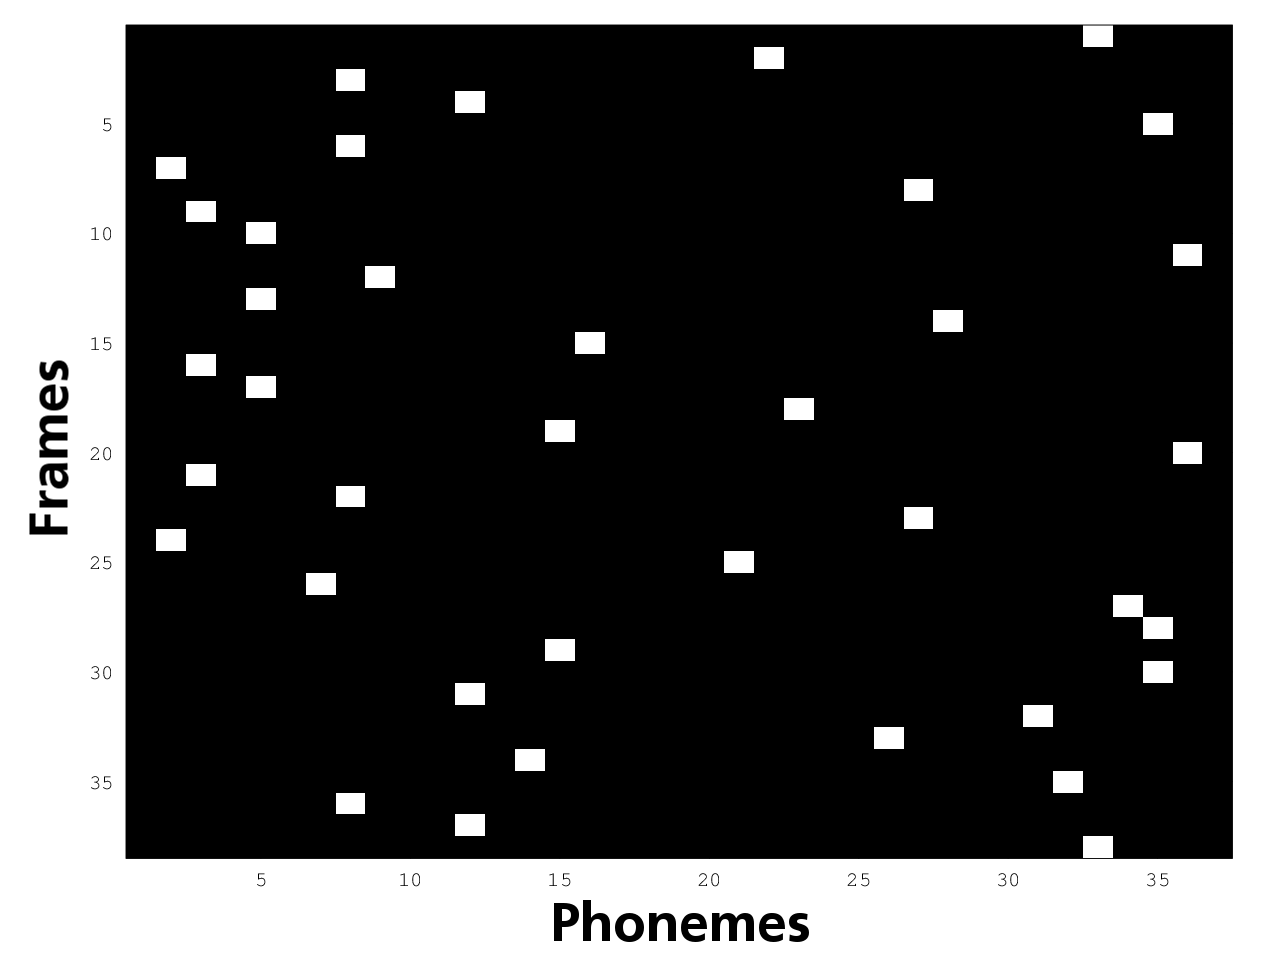
\includegraphics[width=\textwidth]{images/retrieval_template.png}
		\caption{Phoneme template}
	\end{subfigure}

	\begin{subfigure}[t]{0.3\textwidth}
		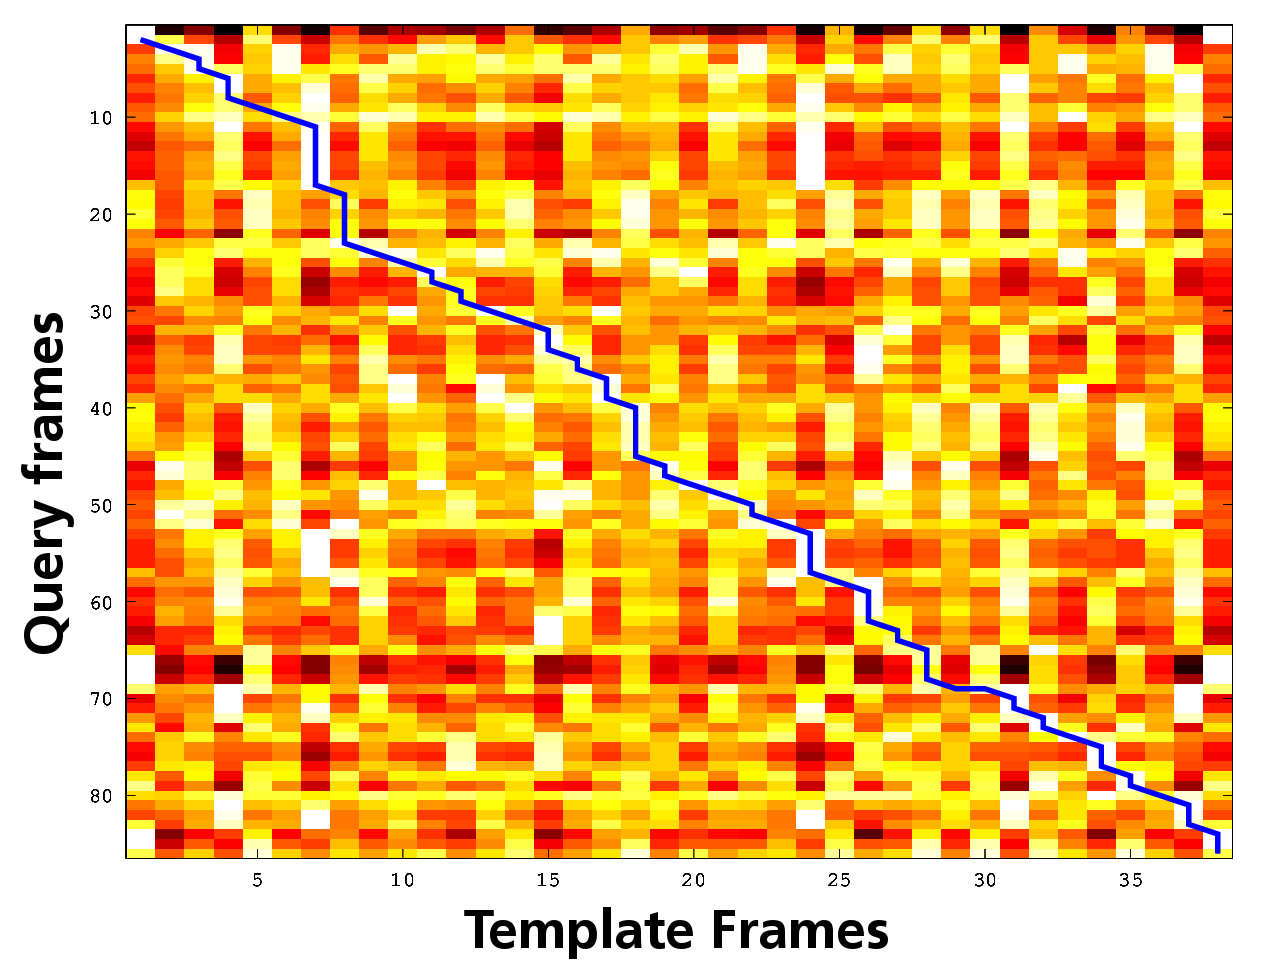
\includegraphics[width=\textwidth]{images/retrieval_similarity.png}
		\caption{Similarity matrix with cheapest path (blue)}
	\end{subfigure}
	\caption{Example of a similarity calculation: Phoneme posteriorgrams are calculated for the audio recordings \textbf{(a)}. Phoneme templates are generated for the textual lyrics \textbf{(b)}. Then, a similarity matrix is calculated using the cosine distance between the two, and DTW is performed on it \textbf{(c)}. The accumulated cost divided by the path length is the similarity measure.}\label{fig:retrieval_dtw}
\end{figure}

\subsection{Alignment experiments}
\ref{fig:results_align_dtw}

\begin{figure}
 \begin{center}
                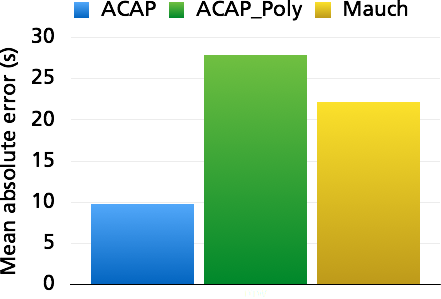
\includegraphics[width=0.8\textwidth]{images/res_align_dtw.png}
               \caption{\textit{MIREX} results on all three data sets using the DTW-based approach.}
                \label{fig:results_align_dtw}
                 \end{center}
 \end{figure}



\subsection{Retrieval experiments on whole song inputs}
In the first experiment, similarity measures were calculated between the lyrics and recordings of whole songs using the described process. This was tested with phoneme posteriorgrams obtained with all five acoustic models on the female and the male test sets (\textit{DampTestF} and \textit{DampTestM}). The accuracy was then calculated on the 1-, 3-, and 10-best results for each song (i.e., how many lyrics are correctly detected when taking into account the 1, 3, and 10 lowest distances?). The results on the female test set are shown in figure \ref{fig:retrieval_dtwres_testF}, the ones for the male test set in figure \ref{fig:retrieval_dtwres_testM}.

\begin{figure}
       \centering
        \begin{subfigure}[b]{0.3\textwidth}
	    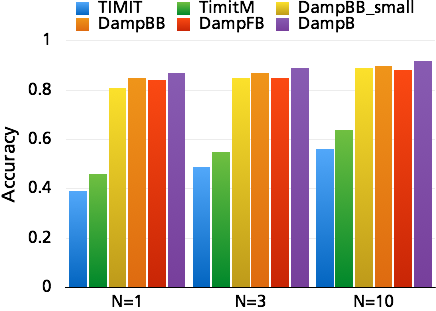
\includegraphics[width=\textwidth]{images/retrieval_dtwres_testF.png}
                \caption{DampTestF}
                \label{fig:retrieval_dtwres_testF}
        \end{subfigure}%
         %add desired spacing between images, e. g. ~, \quad, \qquad, \hfill etc.
          %(or a blank line to force the subfigure onto a new line)
         \vspace{10px}
        \begin{subfigure}[b]{0.3\textwidth}
	  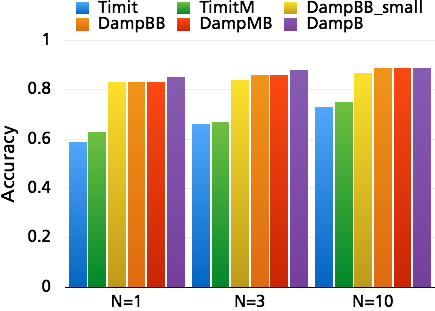
\includegraphics[width=\textwidth]{images/retrieval_dtwres_testM.png}
                \caption{DampTestM}
                \label{fig:retrieval_dtwres_testM}
        \end{subfigure}

        \caption{Accuracies of the results for lyrics detection on the whole song for the \textit{DampTest} sets using five different acoustic models, and evaluated on the 1-, 3-, 10-, 50-, and 100-best results.}\label{fig:retrieval_dtwres}
\end{figure}

 These results show that phoneme posteriorgrams obtained with models trained on speech data (\textit{TIMIT}) generally produce the lowest results in lyrics retrieval. The difference between the two test sets is especially interesting here: On the male test set, the accuracy for the single best result is $58\%$, while on the female set it is only $39\%$. Previous experiments showed that the phoneme recognition itself performs somewhat worse for female singing inputs. This effect is compounded in these lyrics retrieval results. This may happen because the frequency range of female singing is even further removed from that of speech than the frequency range of male singing is \cite{sundberg}. Even female speech is often performed at the lower end of the female singing frequency range. The frequency range of male singing is better covered when training models on speech recordings (especially when speech recordings of both genders are used).\\
 This effect is still visible for the \textit{TimitM} models, which is the variant of \textit{Timit} that was artificially made more ``song-like''. However, the pitch range was not expanded too far in order to keep the sound natural.\\
The results improve massively when acoustic models trained on any of the \textit{DAMP} singing corpora are used. The difference between the male and female results disappears, which supports the idea that the female pitch range was not covered well by the models trained on speech. Using the models trained on the smallest singing data set (\textit{DampBB\_small}), which is slightly smaller than \textit{Timit}, the results increase to $81\%$ and $83\%$ for the single best result on the female and the male test set respectively. With the models trained on the \textit{DampBB} corpus, which is about twice as big, they increase slightly more to $85\%$ on the female test set. Gender-specific models of the same size do not improve the result in this case.\\
Finally, the results obtained with the acoustic models trained on the largest singing corpus (\textit{DampB}) provide the very best results at accuracies of $87\%$ and $85\%$.\\
For some applications, working with the best N instead of just the very best result could be useful (e.g. for presenting a selection of possible lyrics to a user). When the best 3 results can be taken into account, the accuracies on the best posteriorgrams rise to $89\%$ and $88\%$ on the female and male test sets respectively. When the best 10 results are used, they reach $92\%$ and $89\%$.

\subsection{Lyrics retrieval experiments on line-wise inputs}
\vspace{-2px}
In the second retrieval experiment, the same process was performed on single lines of sung lyrics as inputs (usually a few seconds in duration). Costs were then calculated between the posteriorgrams of these recordings and all 12,000 available lines of lyrics. Lines with fewer than 10 phonemes were not taken into account.\\
Then, evaluation was performed as to whether a line from the correct song was retrieved in the N-best results. In this way, confusions between repetitions of a line in the same song did not have an impact on the result. However, repetitions of lyrical lines across multiple songs are a possible source of confusion. The results for the female test set are shown in figure \ref{fig:retrieval_dtwres_testF_line}, the ones for the male test set in figure \ref{fig:retrieval_dtwres_testM_line}.
\setlength{\belowcaptionskip}{-0.3cm}
\begin{figure}
        \centering
        \begin{subfigure}[b]{0.3\textwidth}
	    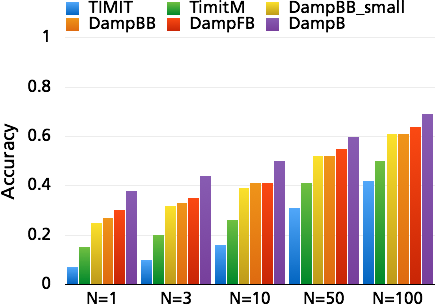
\includegraphics[width=\textwidth]{images/retrieval_dtwres_testF_line.png}
                \caption{DampTestF}
                \label{fig:retrieval_dtwres_testF_line}
        \end{subfigure}%
        %add desired spacing between images, e. g. ~, \quad, \qquad, \hfill etc.
          %(or a blank line to force the subfigure onto a new line)
          \vspace{10px}
       \begin{subfigure}[b]{0.3\textwidth}
	  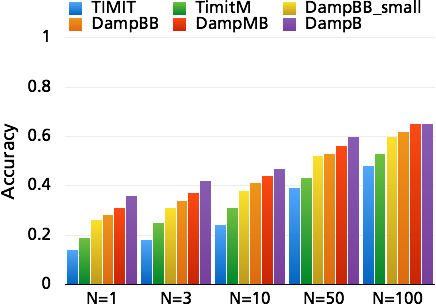
\includegraphics[width=\textwidth]{images/retrieval_dtwres_testM_line.png}
                \caption{DampTestM}
                \label{fig:retrieval_dtwres_testM_line}
       \end{subfigure}
        \setlength{\belowcaptionskip}{-0.6cm}
        \caption{Accuracies of the results for lyrics detection on separate lines of sung lyrics for the \textit{DampTest} sets using five different acoustic models, and evaluated on the 1-, 3-, 10-, 50-, and 100-best results.}\label{fig:retrieval_dtwres_line}
\end{figure}

Again, a difference between both test sets is visible when generating posteriograms with the \textit{TIMIT} models. The accuracy on the best result is $14\%$ for the male test set, but just $7\%$ for the female test.\\
The results for the \textit{DAMP} models show the same basic tendencies as before, although naturally much lower. For the single best result, the accuracies when using the \textit{DampB} model are $38\%$ and $36\%$ on the female and male test sets respectively. For this task, gender-dependent models produce slightly higher results than the mixed-gender ones of the same size.\\



\section{Phoneme-based retrieval and alignment}
Next, another step was introduced to improve the previous approach and make it more flexible. This step serves to compress the posteriorgrams down to a plausible sequence of phonemes, which can then be used to search directly on a textual lyrics database. Text comparison is much cheaper than the previous comparison strategy, and enables quick expansion of the lyrics database.\\
In parallel, the lyrics database is prepared by converting it into phoneme sequences as described in section \ref{}. The key algorithms are (a) how to generate plausible phoneme sequences from the posteriorgrams, and (b) how to compare these against the sequences in the database. These parts will be described in more detail in the following. An overview is given in figure \ref{fig:retrieval_phone_overview}.

%TODO: phoneme seqs erkl�ren
\begin{figure}
 \begin{center}
                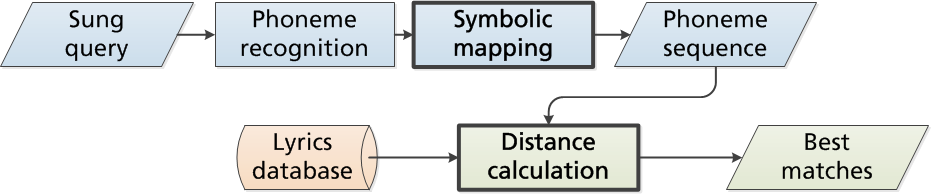
\includegraphics[width=.45\textwidth]{images/retrieval_phone_overview.png}
                \caption{Overview of the phoneme-based lyrics retrieval process.}
                \label{fig:retrieval_phone_overview}
                 \end{center}
 \end{figure}

\vspace{-5pt}
\paragraph{Symbolic mapping}
As described before, starting from the sung recording used as a query, MFCC features are extracted and run through the acoustic model trained on singing to recognize the contained phonemes. This produces a phoneme posteriorgram, such as the one shown in figure \ref{fig:posteriorgram}; i.e., probabilities of each phone over each time frame. These probabilities contain some noise, both due to inaccuracies in the model and due to ambiguities or actual noise in the performance.\\ %Why not HMMSs??
The following steps are undertaken to obtain a plausible phoneme sequence from the posteriorgram:
\begin{description}
	\item[Smoothing] First, the posteriorgram is smoothed along the time axis with a window of length 3 in order to remove small blips in the phoneme probabilities. 
	\item[Maximum selection and grouping] Then, the maximum bin (i.e. phoneme) per frame is selected, and consecutive results are grouped. An example is given in figure \ref{fig:retrieval_phone_block1}.
	\item[Filtering by probability and duration] These results can then be pre-filtered to discard those that are too short or to improbable. This is done with different parameterizations for vowels and consonants since vowels are usually longer in duration. This yields a first sequence of phonemes, each with duration and sum probability information, which is usually too long and noisy. In particular, a lot of fluctuations between similar phonemes occur. %; an example is shown in figure \ref{fig:}.
	\item[Grouping by blocks and filtering through confusion matrix] This problem is solved by first grouping the detected phonemes into blocks, in this case vowel and consonant blocks (shown in figure \ref{fig:block2}). Then, a decision needs to be made as to which elements of these blocks are the ``true'' phonemes and which ones are noise. This is done by taking each phoneme's probability as well as the confusion between phonemes into account. The confusion is calculated in advance by running the classifier on an annotated test set; the result covers both the confusion by inaccuracies in the classifier as well as perceptual or performance-based confusions (e.g. transforming a long \textit{[ay]} sound into \textit{[aa - ay - iy]} during singing). An example is shown in figure \ref{fig:retrieval_phone_confusion}. The product of the probabilities and the confusions are calculated for the highest combinations up to a certain threshold, and all other detected phonemes are discarded. This results in a shorter, more plausible phoneme sequence (figure \ref{fig:retrieval_phone_block3}).% such as the example shown in figure \ref{fig:}.
\end{description}
%listing?

  \begin{figure}
  \setlength{\belowcaptionskip}{0pt}

	\centering
	\begin{subfigure}[t]{0.25\textwidth}
		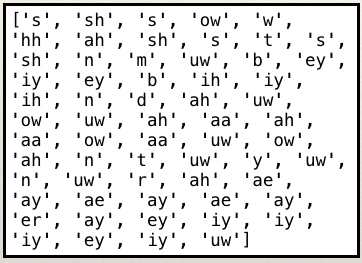
\includegraphics[width=.8\textwidth]{images/retrieval_phone_block1.png}
		\caption{Original phoneme sequence}\label{fig:retrieval_phone_block1}
	\end{subfigure}%
	\begin{subfigure}[t]{0.3\textwidth}
		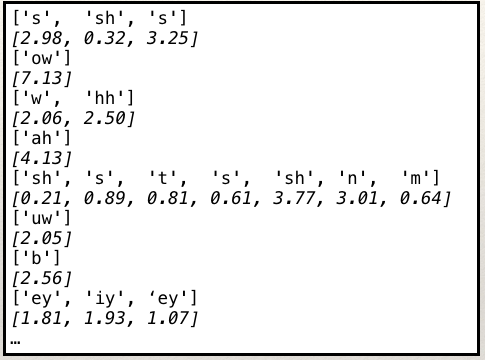
\includegraphics[width=.8\textwidth]{images/retrieval_phone_block2.png}
		\caption{Grouped into blocks (with probabilities in italics)}\label{fig:retrieval_phone_block2}
	\end{subfigure}
	\begin{subfigure}[t]{0.25\textwidth}
		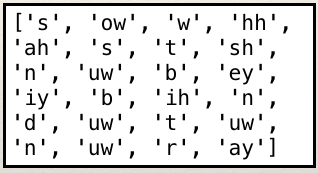
\includegraphics[width=.8\textwidth]{images/retrieval_phone_block3.png}
		\caption{Filtered result}\label{fig:retrieval_phone_block3}
	\end{subfigure}
	\setlength{\belowcaptionskip}{-10pt}

	\caption{Example of the block grouping of the phoneme sequence and subsequent filtering by probabilities and confusions.}\label{fig:retrieval_phone_blocking}
\end{figure}

\begin{figure}
	\begin{center}
		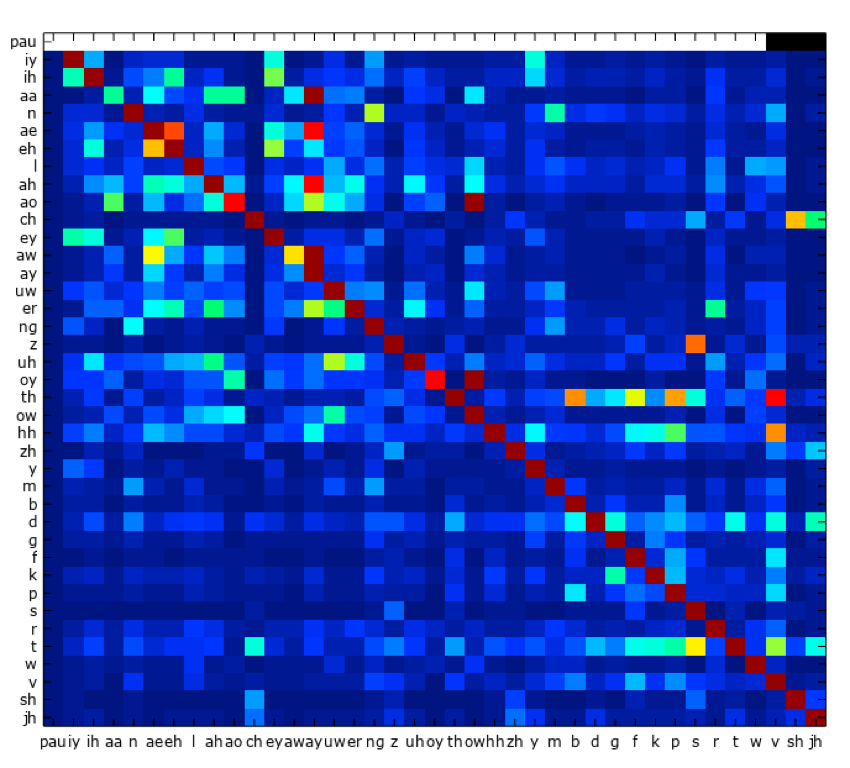
\includegraphics[width=.45\textwidth]{images/retrieval_phone_confusion.png}
		\caption{Example of a confusion matrix for an acoustic model. (Note that \textit{[pau]} confusions are set to 0).}
		\label{fig:retrieval_phone_confusion}
	\end{center}
\end{figure}

\begin{table}[h!tp]
\footnotesize
\begin{center}
\begin{tabular}{|c||c|c|c||c|c|c||c|c|c|}
\hline
 & \multicolumn{3}{|c|}{Female} & \multicolumn{3}{|c|}{Male} & \multicolumn{3}{|c|}{Author} \\
 & Top1 & Top3 & Top10 & Top1 & Top3 & Top10 & Top1 & Top3 & Top10 \\
\hline \hline
Baseline & .25 & .25 & .35 & .1 & .1 & .2 & .1 &.23 &.36 \\
\hline
Posteriorgram smoothing & .65 & .7 & .90 & .5 & .65 &.65 &.61 &.67 &.76 \\
\hline
Filtering blocks by probabilities and confusions & .8 & .85 &.96 & .75 &.8 &.85 &.74 &.78 &.82 \\
\hline
Substitution weights & .9 &.95 &.95 &.65 &.8 &.9 &.76 &.78 &.83 \\
\hline
Substitution + Insertion weights & 1 & 1 & 1 & .75 & .85 &.9 &.81 &.84 &.9 \\
\hline
\end{tabular}
\end{center}
\caption{Results of the retrieval algorithm for three test data sets with various improvement steps.}
\label{tab:results}
\end{table}%

\vspace{-5pt}
\paragraph{Distance calculation} 
Then, the distances between the extracted phoneme sequence and the ones provided in the lyrics database are calculated.\\
First, an optional step to speed up the process is introduced. Each sequence's number of vowels is counted in advance, and the same is done for the query sequence. Then, only sequences with roughly the same amount of vowels are compared (with some tolerance). This slightly decreases accuracies, but drastically speeds up the calculation time.\\
The similarity calculation itself is implemented with a modified Levenshtein distance. Again, the classifier's confusion between phonemes is taken into account. These confusions are used as the Levenshtein weights for substitutions. Surprisingly, using them for insertion weights improves the results as well. This probably happens because of the effect described above: A singer will in many cases vocalize an phoneme as multiple different ones, particularly for vowels with long durations. This will result in an insertion in the detected phoneme sequence, which is not necessarily a ``wrong'' classification by the acoustic model, but does not correspond to the expected sequence for this line of lyrics. For this reason, such insertions should not be harshly penalized. For deletions, the weight is set to $.5$ to balance out the lower insertion and substitution weights.



\subsection{Alignment experiments}
\ref{fig:results_align_phone}
\begin{figure}
 \begin{center}
                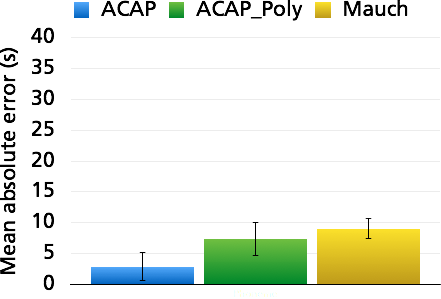
\includegraphics[width=0.8\textwidth]{images/res_align_phone.png}
               \caption{\textit{MIREX} results on all three data sets using the phoneme-based approach.}
                \label{fig:results_align_phone}
                 \end{center}
 \end{figure}

%TODO: same eval data...
\subsection{Experiments and results}
Table \ref{tab:results} shows an overview over the experimental results. We tested the approach on the three test sets described in section \ref{sec:data} and report the retrieval rates for the Top 1 result (i.e. the one with the lowest Levenshtein distance), the Top 3, and the Top 10 results. Queries were allowed to be one to three consecutive lines of songs, increasing the number of ``virtual'' database entries to around 36,000 (12,000 lines as 1-, 2-, and 3-grams). It should be noted that a result counts as correct when the correct song (out of 300) was detected; this was done as a simplification because the same line of lyrics is often repeated in songs. For possible applications, users are most probably interested in obtaining the correct full song lyrics, rather than a specific line. Picking random results would therefore result in a retrieval rate of $.003$.\\
We then tested the various improvement steps of the algorithm as follows:
\begin{description}
\item[Baseline] As a baseline system, we used the most straightforward approach: Directly pick the phonemes with the highest probabilities for each frame from the posteriorgram, group them by consecutive phonemes, and use the result of that for searching the lyrics database with a standard Levenshtein implementation. This results in retrieval rates of $.25$, $.1$, and $.23$ for the Female, Male, and Author test sets respectively.
\item[Posteriorgram smoothing] This is the same as the baseline approach, but we smooth the posteriorgram along the time axis as described in section \ref{subsec:mapping}. This already improves the result by around $.4$ for each test set.
\item[Filtering blocks by probabilities and confusions] This includes the last step described in section \ref{subsec:mapping}. The result is improved further by $.13$ to $.25$.
\item[Substitution and insertion weights] Finally, we use the modified Levenshtein distance as described in section \ref{subsec:distance}. When using the confusion weights for phoneme substitutions only, the result increases further, and even more so when they are also used for the insertion weights. The final Top 1 retrieval rates are $1$, $.75$, and $.81$ for the three test sets respectively.
\end{description}




\section{Application: Expletive detection}

Lots of song lyrics contain expletives. There are many scenarios in which it is necessary to know when these words occur, e.g. for airplay and for the protection of minors. In the case of airplay, they are commonly ``bleeped" or acoustically removed. The alignment strategies described previously are employed for the practical scenario of finding such expletives automatically.\\
The test data set is the one compiled by Queen Mary University, described in section \ref{subsec:data_qmul}.\\

A direct keyword spotting approach was also considered, but this did not generate sufficient results since most of the expletives only consist of 2 or 3 phonemes. Keyword spotting becomes notoriously hard for such short keywords as described in chapter \ref{chap:kws}.\\
Since textual lyrics are usually easily available on the internet, a new approach utilizing those was developed:
\begin{enumerate}
\item Automatically align textual lyrics to audio (as described above)
\item Search for pre-defined expletives in the result
\item If necessary, remove those expletives. A stereo subtraction approach was used, which works adequately for this case since the removed timespans are short. Alternatively, keywords can be masked with a bleep or similar.
\end{enumerate}
The data flow is shown in figure \ref{fig:expletive_dataflow}.
\begin{figure}
\begin{center}
                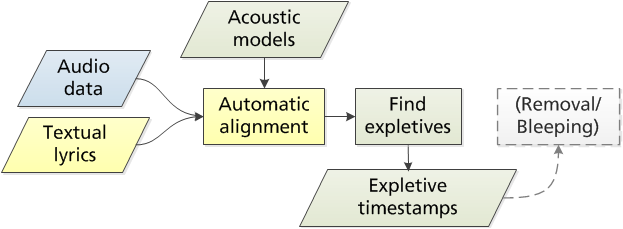
\includegraphics[width=0.4\textwidth]{images/expletive_approach.png}
                \caption{Data flow in the expletive detection approach.}
                \label{fig:expletive_dataflow}
                 \end{center}
 \end{figure}

The alignment was performed using the HMM-based alignment described in section \ref{sec:ret_hmm}, and the DTW alignment from section \ref{sec:ret_post} using the DNN acoustic models trained on \textit{TIMIT} and on \textit{DampB}. Accuracy was then calculated by evaluating how many of the annotated expletives were recognized at their correct timestamps (with various tolerances). The results are shown in figure \ref{fig:expletive_results}.
\begin{figure}
 \begin{center}
                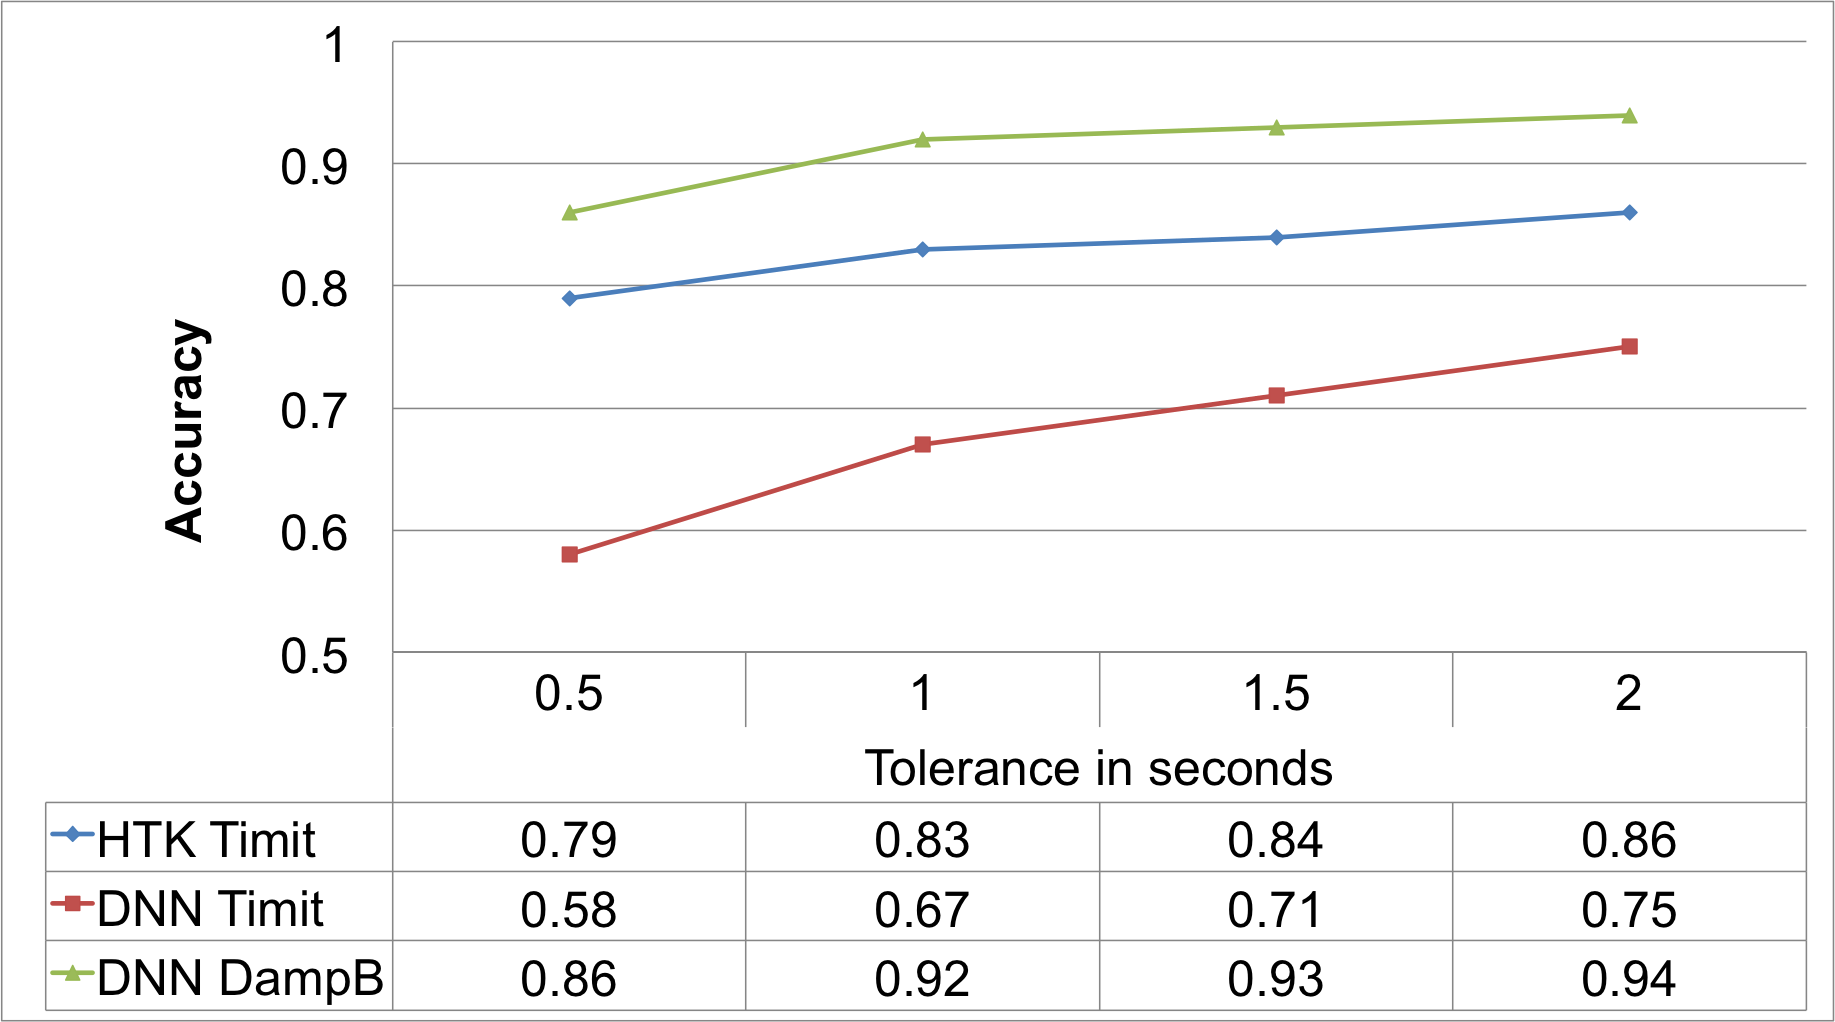
\includegraphics[width=0.4\textwidth]{images/expletive_results.png}
               \caption{Results for the expletive detection approach at various tolerances.}
                \label{fig:expletive_results}
                 \end{center}
 \end{figure}
 %analyze?

In this small practical example, only two alignment strategies were tested, but there are others that could provide better results. Whenever the alignment failed, it was mostly due to solo instruments. In order to remedy this, vocal detection (and possibly source separation) could be employed prior to alignment. Additionally, a more sophisticated removal approach could be implemented to remove the expletives.\\
Lyrics collected from the internet are often incorrect, e.g. because repetitions are not spelled out, because of spelling errors, or because they refer to different versions of a song. This approach could be expanded to allow for some flexibility in this respect. At the moment, these lyrics need to be provided manually. In the future, those could be retrieved automatically (e.g. using the approaches described above).\\


%TODO: Clean up!
\section{Conclusion}
%error sources: same as mentioned in phonerec because same data!!
%error source: amateur recordings
In this paper, we presented an approach to retrieving the matching lyrics for a singing recording from a fixed database of 300 textual lyrics. To do this, we first extract phoneme posteriorgrams from the audio and generate phoneme templates from all possible lyrics. We then perform Dynamic Time Warping on all combinations to obtain distance measures.\\
When the whole song is used as the input, we obtain an accuracy of $86\%$ for the single best result. If the 10 best results are taken into account, this rises to $91\%$. When using only short sung lines as input, the mean 1-best accuracy for retrieving the correct song lyrics of the whole song is $37\%$. For the best 100 results, the accuracy is $67\%$.\\
An interesting result was the difference between the female and the male test sets: On the female test set, retrieval with models trained on speech was significantly lower than on the male set ($39\%$ vs. $58\%$ on the song-wise task). We believe this happens because the frequency range of female singing is not covered well with speech data only. When using acoustic models trained on singing, this difference disappears and the results become significantly higher in general. Even for a model trained on less data than that contained in \textit{Timit}, the average accuracy is $82\%$.\\
When looking at possible sources of error, many of them had to do with enunciation issues (clarity, accents, or children's voices) or issues with the recording itself (background music, clipping, extraneous speaking). These problems would not be as prevalent in professional recordings. However, some of them could be fixed with adaptations to the algorithm.

As mentioned before, we would like to improve our algorithm to be more robust to the detected error sources. Other possible points of improvement include the choice of the distance metric or of the acoustic models. Preliminary tests suggest that combining results of different phoneme recognizers could improve the over-all result.\\
We have not tested this approach on singing with background music yet, which could be an interesting next step. So far, only a fixed corpus of possible lyrics was taken into account. Opening the approach up to larger databases would make it more flexible. This could be combined with Semantic Web technologies to automatically find lyrics on the internet.\\
When the space of possible lyrics becomes larger, techniques for scalability will be necessary. One such idea could be a rough search with smaller lyrical ``hashes'' to find possible matches, and then a refinement with our current approach. This is similar to techniques that are already used in audio fingerprinting \cite{shazam}.


In this paper, we presented a new approach for retrieving textual lyrics from single lines of sung queries. To this end, we first extract phoneme posteriorgrams from the audio recording with acoustic models trained on a large singing database. Then, we employ a new algorithm to map the result to a symbolic representation (i.e. a phoneme sequence). This sequence is then compared to the ones in the lyrics database using a modified Levenshtein distance.\\
We found several improvements to this basic algorithm. First, we noticed that smoothing the posteriorgram along the time axis with a short window removes spurious probability fluctuations. The mapping from the posteriorgram to the symbolic representation can be improved by filtering the phonemes with the highest probabilities with the known phoneme confusions. Finally, we modified the Levenshtein distance by also utilizing these confusions for substitution and insertion weights. The final results range between $.75$ and $1$ for the Top 1 result, and between $.9$ and $1$ for the Top 10.

In the next step, we would like to perform a more extensive evaluation of the various components of the algorithm. In particular, it would be interesting to research the relationship between retrieval rate and the number of phonemes in the query in more detail. Related to this, we would like to evaluate the approach for speeding up the search by filtering by number of vowels more closely.\ As mentioned in section \ref{sec:approach}, HMMs are an alternative for obtaining the phoneme sequence from the posteriorgram which would be interesting to test.\\
%The suggested approach can be integrated into various systems as described in section \ref{sec:intro}; one particularly interesting application is the search of lyrics on the internet without a prepared database. Our method could be expanded to enable this. Additionally, the described algorithm can also be employed for lyrics-to-singing alignment by calculating the Levenshtein alignment between the detected and the expected phoneme sequence. This algorithm performed best at 2017's \textit{MIREX} challenge for lyrics-to-audio alignment\footnote{\url{http://www.music-ir.org/mirex/wiki/2017:Automatic_Lyrics-to-Audio_Alignment_Results}}.
